% Options for packages loaded elsewhere
\PassOptionsToPackage{unicode}{hyperref}
\PassOptionsToPackage{hyphens}{url}
%
\documentclass[
]{book}
\usepackage{amsmath,amssymb}
\usepackage{iftex}
\ifPDFTeX
  \usepackage[T1]{fontenc}
  \usepackage[utf8]{inputenc}
  \usepackage{textcomp} % provide euro and other symbols
\else % if luatex or xetex
  \usepackage{unicode-math} % this also loads fontspec
  \defaultfontfeatures{Scale=MatchLowercase}
  \defaultfontfeatures[\rmfamily]{Ligatures=TeX,Scale=1}
\fi
\usepackage{lmodern}
\ifPDFTeX\else
  % xetex/luatex font selection
\fi
% Use upquote if available, for straight quotes in verbatim environments
\IfFileExists{upquote.sty}{\usepackage{upquote}}{}
\IfFileExists{microtype.sty}{% use microtype if available
  \usepackage[]{microtype}
  \UseMicrotypeSet[protrusion]{basicmath} % disable protrusion for tt fonts
}{}
\makeatletter
\@ifundefined{KOMAClassName}{% if non-KOMA class
  \IfFileExists{parskip.sty}{%
    \usepackage{parskip}
  }{% else
    \setlength{\parindent}{0pt}
    \setlength{\parskip}{6pt plus 2pt minus 1pt}}
}{% if KOMA class
  \KOMAoptions{parskip=half}}
\makeatother
\usepackage{xcolor}
\usepackage{color}
\usepackage{fancyvrb}
\newcommand{\VerbBar}{|}
\newcommand{\VERB}{\Verb[commandchars=\\\{\}]}
\DefineVerbatimEnvironment{Highlighting}{Verbatim}{commandchars=\\\{\}}
% Add ',fontsize=\small' for more characters per line
\usepackage{framed}
\definecolor{shadecolor}{RGB}{248,248,248}
\newenvironment{Shaded}{\begin{snugshade}}{\end{snugshade}}
\newcommand{\AlertTok}[1]{\textcolor[rgb]{0.94,0.16,0.16}{#1}}
\newcommand{\AnnotationTok}[1]{\textcolor[rgb]{0.56,0.35,0.01}{\textbf{\textit{#1}}}}
\newcommand{\AttributeTok}[1]{\textcolor[rgb]{0.13,0.29,0.53}{#1}}
\newcommand{\BaseNTok}[1]{\textcolor[rgb]{0.00,0.00,0.81}{#1}}
\newcommand{\BuiltInTok}[1]{#1}
\newcommand{\CharTok}[1]{\textcolor[rgb]{0.31,0.60,0.02}{#1}}
\newcommand{\CommentTok}[1]{\textcolor[rgb]{0.56,0.35,0.01}{\textit{#1}}}
\newcommand{\CommentVarTok}[1]{\textcolor[rgb]{0.56,0.35,0.01}{\textbf{\textit{#1}}}}
\newcommand{\ConstantTok}[1]{\textcolor[rgb]{0.56,0.35,0.01}{#1}}
\newcommand{\ControlFlowTok}[1]{\textcolor[rgb]{0.13,0.29,0.53}{\textbf{#1}}}
\newcommand{\DataTypeTok}[1]{\textcolor[rgb]{0.13,0.29,0.53}{#1}}
\newcommand{\DecValTok}[1]{\textcolor[rgb]{0.00,0.00,0.81}{#1}}
\newcommand{\DocumentationTok}[1]{\textcolor[rgb]{0.56,0.35,0.01}{\textbf{\textit{#1}}}}
\newcommand{\ErrorTok}[1]{\textcolor[rgb]{0.64,0.00,0.00}{\textbf{#1}}}
\newcommand{\ExtensionTok}[1]{#1}
\newcommand{\FloatTok}[1]{\textcolor[rgb]{0.00,0.00,0.81}{#1}}
\newcommand{\FunctionTok}[1]{\textcolor[rgb]{0.13,0.29,0.53}{\textbf{#1}}}
\newcommand{\ImportTok}[1]{#1}
\newcommand{\InformationTok}[1]{\textcolor[rgb]{0.56,0.35,0.01}{\textbf{\textit{#1}}}}
\newcommand{\KeywordTok}[1]{\textcolor[rgb]{0.13,0.29,0.53}{\textbf{#1}}}
\newcommand{\NormalTok}[1]{#1}
\newcommand{\OperatorTok}[1]{\textcolor[rgb]{0.81,0.36,0.00}{\textbf{#1}}}
\newcommand{\OtherTok}[1]{\textcolor[rgb]{0.56,0.35,0.01}{#1}}
\newcommand{\PreprocessorTok}[1]{\textcolor[rgb]{0.56,0.35,0.01}{\textit{#1}}}
\newcommand{\RegionMarkerTok}[1]{#1}
\newcommand{\SpecialCharTok}[1]{\textcolor[rgb]{0.81,0.36,0.00}{\textbf{#1}}}
\newcommand{\SpecialStringTok}[1]{\textcolor[rgb]{0.31,0.60,0.02}{#1}}
\newcommand{\StringTok}[1]{\textcolor[rgb]{0.31,0.60,0.02}{#1}}
\newcommand{\VariableTok}[1]{\textcolor[rgb]{0.00,0.00,0.00}{#1}}
\newcommand{\VerbatimStringTok}[1]{\textcolor[rgb]{0.31,0.60,0.02}{#1}}
\newcommand{\WarningTok}[1]{\textcolor[rgb]{0.56,0.35,0.01}{\textbf{\textit{#1}}}}
\usepackage{longtable,booktabs,array}
\usepackage{calc} % for calculating minipage widths
% Correct order of tables after \paragraph or \subparagraph
\usepackage{etoolbox}
\makeatletter
\patchcmd\longtable{\par}{\if@noskipsec\mbox{}\fi\par}{}{}
\makeatother
% Allow footnotes in longtable head/foot
\IfFileExists{footnotehyper.sty}{\usepackage{footnotehyper}}{\usepackage{footnote}}
\makesavenoteenv{longtable}
\usepackage{graphicx}
\makeatletter
\newsavebox\pandoc@box
\newcommand*\pandocbounded[1]{% scales image to fit in text height/width
  \sbox\pandoc@box{#1}%
  \Gscale@div\@tempa{\textheight}{\dimexpr\ht\pandoc@box+\dp\pandoc@box\relax}%
  \Gscale@div\@tempb{\linewidth}{\wd\pandoc@box}%
  \ifdim\@tempb\p@<\@tempa\p@\let\@tempa\@tempb\fi% select the smaller of both
  \ifdim\@tempa\p@<\p@\scalebox{\@tempa}{\usebox\pandoc@box}%
  \else\usebox{\pandoc@box}%
  \fi%
}
% Set default figure placement to htbp
\def\fps@figure{htbp}
\makeatother
\setlength{\emergencystretch}{3em} % prevent overfull lines
\providecommand{\tightlist}{%
  \setlength{\itemsep}{0pt}\setlength{\parskip}{0pt}}
\setcounter{secnumdepth}{5}
\usepackage{booktabs}
\usepackage{amsthm}
\makeatletter
\def\thm@space@setup{%
  \thm@preskip=8pt plus 2pt minus 4pt
  \thm@postskip=\thm@preskip
}
\makeatother
\usepackage[]{natbib}
\bibliographystyle{apalike}
\usepackage{bookmark}
\IfFileExists{xurl.sty}{\usepackage{xurl}}{} % add URL line breaks if available
\urlstyle{same}
\hypersetup{
  pdftitle={Análisis de Series de Tiempo para la Predicción de Precios de Acciones},
  pdfauthor={Julian Rojas y Natalia Tangarife},
  hidelinks,
  pdfcreator={LaTeX via pandoc}}

\title{Análisis de Series de Tiempo para la Predicción de Precios de Acciones}
\author{Julian Rojas y Natalia Tangarife}
\date{2025-10-13}

\begin{document}
\maketitle

{
\setcounter{tocdepth}{1}
\tableofcontents
}
\chapter*{Propuesta de Análisis}\label{propuesta-de-anuxe1lisis}
\addcontentsline{toc}{chapter}{Propuesta de Análisis}

\section{Descripción de la Información}\label{descripciuxf3n-de-la-informaciuxf3n}

Para este curso trabajaremos con \textbf{series de tiempo de precios diarios de acciones} de empresas tecnológicas cotizadas en mercados estadounidenses, específicamente de compañías como Apple (AAPL), Microsoft (MSFT) y Tesla (TSLA). Los datos incluyen precios de cierre, apertura, máximos, mínimos y volúmenes de negociación, capturados a través de la librería \texttt{quantmod} que accede a \textbf{Yahoo Finance}.

La serie temporal abarca el período \textbf{2015-2025 (últimos 10 años)}, proporcionando aproximadamente \textbf{2,500 observaciones por activo}. Este período es particularmente valioso porque incluye:

\begin{itemize}
\tightlist
\item
  \textbf{Pre-pandemia (2015-2019):} Período de crecimiento estable y expansión económica
\item
  \textbf{Crisis COVID-19 (2020-2021):} Caída abrupta del mercado en marzo 2020 y posterior recuperación acelerada
\item
  \textbf{Post-pandemia (2022-2025):} Nuevas dinámicas de mercado, inflación y ajustes de tasas de interés
\end{itemize}

Esta ventana temporal permite analizar cómo las series de tiempo se comportan ante choques externos extremos, cambios de volatilidad drásticos y diferentes regímenes de mercado.

\section{Justificación e Importancia del Pronóstico}\label{justificaciuxf3n-e-importancia-del-pronuxf3stico}

\subsection{El Problema}\label{el-problema}

Los mercados financieros son inherentemente volátiles y presentan comportamientos complejos que combinan tendencias, estacionalidad y componentes aleatorios. Esta complejidad se intensifica dramáticamente durante crisis globales, como lo evidenció el COVID-19 cuando:

\begin{itemize}
\tightlist
\item
  Los mercados experimentaron caídas del 30-40\% en semanas (crash de marzo 2020)
\item
  La volatilidad alcanzó niveles no vistos desde la crisis financiera de 2008
\item
  Las empresas tecnológicas mostraron recuperaciones y crecimientos explosivos
\item
  Los patrones históricos de comportamiento se vieron alterados abruptamente
\end{itemize}

Los inversionistas, analistas y gestores de riesgo necesitan herramientas que les permitan anticipar movimientos de precios incluso en contextos de alta incertidumbre para:

\begin{itemize}
\tightlist
\item
  Optimizar decisiones de compra y venta de activos durante crisis
\item
  Gestionar carteras de inversión de manera proactiva ante cambios de régimen
\item
  Evaluar estrategias de cobertura de riesgo en mercados turbulentos
\item
  Valorar instrumentos derivados considerando volatilidades cambiantes
\end{itemize}

\section{Valor Agregado}\label{valor-agregado}

Este proyecto utiliza \textbf{modelos ARIMA (AutoRegressive Integrated Moving Average)} para pronosticar precios de acciones en horizontes de corto plazo. El valor agregado es particularmente significativo dado el período analizado:

\subsection{1. Análisis de Múltiples Regímenes de Mercado}\label{anuxe1lisis-de-muxfaltiples-reguxedmenes-de-mercado}

Con datos de 2015-2025, podemos evaluar cómo los modelos ARIMA se desempeñan en tres contextos distintos:

\begin{itemize}
\tightlist
\item
  \textbf{Estabilidad (pre-COVID):} Tendencias predecibles y volatilidad moderada
\item
  \textbf{Crisis (COVID-19):} Cambios estructurales abruptos y volatilidad extrema
\item
  \textbf{Recuperación y ajuste:} Nuevas dinámicas post-pandemia
\end{itemize}

\subsection{2. Robustez ante Choques Externos}\label{robustez-ante-choques-externos}

La inclusión del período COVID-19 permite validar si los modelos pueden capturar o adaptarse a disrupciones mayores del mercado, un aspecto crítico que los análisis con datos ``normales'' no pueden evaluar.

\subsection{3. Sector Tecnológico como Caso de Estudio}\label{sector-tecnoluxf3gico-como-caso-de-estudio}

Las empresas seleccionadas (AAPL, MSFT, TSLA) tuvieron comportamientos diferenciados durante la pandemia:

\begin{itemize}
\tightlist
\item
  \textbf{AAPL y MSFT:} Beneficiadas por digitalización acelerada
\item
  \textbf{TSLA:} Crecimiento explosivo a pesar de disrupciones en manufactura
\end{itemize}

Esto permite comparar cómo las series de tiempo reflejan fundamentos empresariales diferentes.

\subsection{4. Aplicación Práctica Dual}\label{aplicaciuxf3n-pruxe1ctica-dual}

\begin{itemize}
\tightlist
\item
  Pronóstico directo de precios para decisiones de trading en contextos de alta/baja volatilidad
\item
  Insumo para valoración mejorada de opciones financieras mediante la combinación ARIMA + Black-Scholes
\end{itemize}

\subsection{5. Cuantificación de Incertidumbre Dinámica}\label{cuantificaciuxf3n-de-incertidumbre-dinuxe1mica}

Los intervalos de confianza generados reflejan cómo la incertidumbre varía según el contexto (ampliándose en crisis, estrechándose en estabilidad).

\subsection{6. Innovación Metodológica}\label{innovaciuxf3n-metodoluxf3gica}

Integrar predicciones ARIMA calibradas con datos que incluyen eventos extremos con modelos de valoración financiera (Black-Scholes) mejora significativamente la estimación de precios de derivados en mercados reales y complejos.

\subsection{Relevancia del Período COVID-19}\label{relevancia-del-peruxedodo-covid-19}

El análisis del período 2020-2021 es especialmente valioso porque representa un \textbf{experimento natural} en finanzas:

\begin{itemize}
\tightlist
\item
  Permite estudiar quiebres estructurales en series de tiempo
\item
  Evalúa la capacidad predictiva de modelos ante eventos de baja probabilidad pero alto impacto (``cisnes negros'')
\item
  Proporciona lecciones sobre adaptación de estrategias de inversión en tiempo real
\item
  Genera insights sobre sectores resilientes vs.~vulnerables en crisis globales
\end{itemize}

\section{Fuentes de Datos y Permisos de Uso}\label{fuentes-de-datos-y-permisos-de-uso}

La información es de carácter público y no requiere permisos especiales, proveniente de Yahoo Finance, una fuente reconocida y confiable en el sector financiero.

\subsection{Especificaciones Técnicas:}\label{especificaciones-tuxe9cnicas}

\begin{itemize}
\tightlist
\item
  \textbf{Fuente principal:} Yahoo Finance a través de la librería \texttt{quantmod} en R
\item
  \textbf{Período de análisis:} 2015-2025 (10 años)
\item
  \textbf{Observaciones:} Aproximadamente 2,500 datos por activo
\item
  \textbf{Frecuencia:} Datos diarios de mercado (252 días por año aproximadamente)
\item
  \textbf{Acceso:} API pública sin restricciones para uso académico y de investigación
\item
  \textbf{Empresas seleccionadas:} Apple (AAPL), Microsoft (MSFT), Tesla (TSLA)
\end{itemize}

\subsection{Variables a Recopilar:}\label{variables-a-recopilar}

\begin{itemize}
\tightlist
\item
  \textbf{Precio de cierre (Close):} Principal variable para modelado de series de tiempo
\item
  \textbf{Precio de apertura (Open):} Para análisis de gaps y volatilidad intradiaria
\item
  \textbf{Precio máximo y mínimo (High/Low):} Para cálculo de rangos y volatilidad
\item
  \textbf{Volumen de negociación:} Indicador de liquidez y confirmación de tendencias
\item
  \textbf{Fechas:} Para construcción de la serie temporal con frecuencia diaria
\end{itemize}

\subsection{Datos Complementarios:}\label{datos-complementarios}

\begin{itemize}
\tightlist
\item
  \textbf{Tasa libre de riesgo:} US Treasury Bills (para modelos de valoración)
\item
  \textbf{Volatilidad implícita:} De mercado de opciones (comparación con volatilidad histórica)
\end{itemize}

\subsection{Consideraciones Legales:}\label{consideraciones-legales}

Todos los datos utilizados provienen de fuentes públicas y gratuitas, destinadas explícitamente para uso académico y de investigación. Yahoo Finance permite el acceso a datos históricos sin restricciones para propósitos educativos. Se citarán adecuadamente todas las fuentes de datos en el análisis final.

\section{Impacto Esperado}\label{impacto-esperado}

El pronóstico preciso de precios mediante series de tiempo que abarcan crisis globales beneficia directamente a:

\begin{itemize}
\tightlist
\item
  \textbf{Inversionistas:} Estrategias informadas sobre cómo activos tecnológicos responden a choques sistémicos
\item
  \textbf{Gestores de riesgo:} Herramientas calibradas con eventos extremos reales, no solo simulaciones
\item
  \textbf{Analistas financieros:} Comprensión profunda de resiliencia sectorial y patrones de recuperación
\item
  \textbf{Académicos e investigadores:} Evidencia empírica sobre comportamiento de series financieras en crisis
\item
  \textbf{Traders de opciones:} Valoración más precisa de instrumentos derivados mediante precios predichos más confiables
\end{itemize}

\begin{center}\rule{0.5\linewidth}{0.5pt}\end{center}

\textbf{Nota}: Este documento constituye la propuesta inicial del proyecto de series de tiempo. A lo largo del curso se desarrollará el análisis completo incluyendo metodología ARIMA, implementación en R, validación de modelos, análisis de residuos, pronósticos y su integración con modelos de valoración de opciones financieras.

\chapter{Introduction}\label{intro}

You can label chapter and section titles using \texttt{\{\#label\}} after them, e.g., we can reference Chapter \ref{intro}. If you do not manually label them, there will be automatic labels anyway, e.g., Chapter \ref{methods}.

Figures and tables with captions will be placed in \texttt{figure} and \texttt{table} environments, respectively.

\begin{Shaded}
\begin{Highlighting}[]
\FunctionTok{par}\NormalTok{(}\AttributeTok{mar =} \FunctionTok{c}\NormalTok{(}\DecValTok{4}\NormalTok{, }\DecValTok{4}\NormalTok{, .}\DecValTok{1}\NormalTok{, .}\DecValTok{1}\NormalTok{))}
\FunctionTok{plot}\NormalTok{(pressure, }\AttributeTok{type =} \StringTok{\textquotesingle{}b\textquotesingle{}}\NormalTok{, }\AttributeTok{pch =} \DecValTok{19}\NormalTok{)}
\end{Highlighting}
\end{Shaded}

\begin{figure}

{\centering 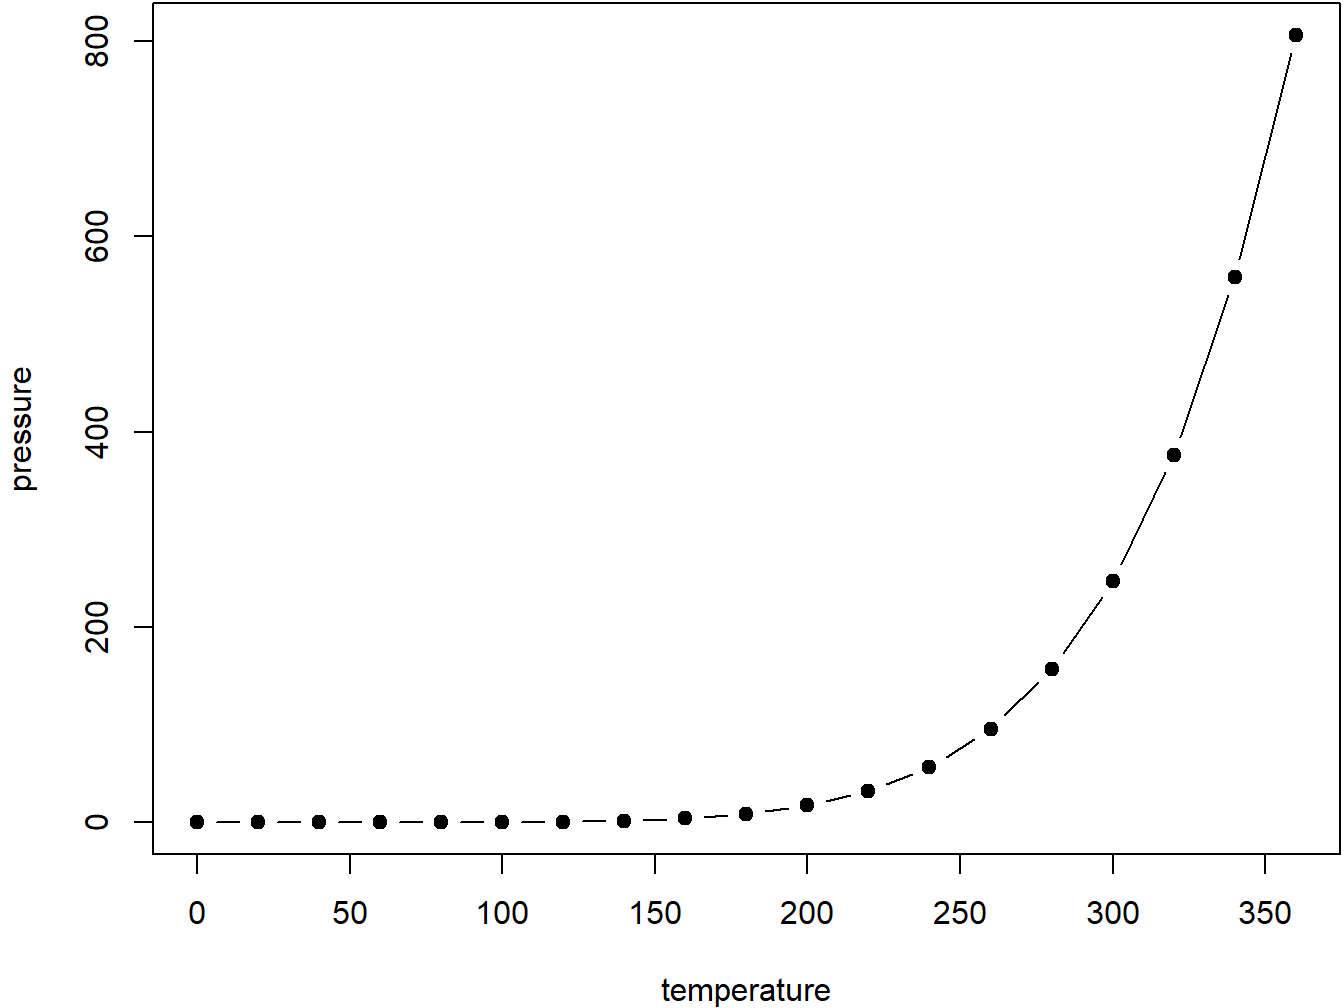
\includegraphics[width=0.8\linewidth]{01-intro_files/figure-latex/nice-fig-1} 

}

\caption{Here is a nice figure!}\label{fig:nice-fig}
\end{figure}

Reference a figure by its code chunk label with the \texttt{fig:} prefix, e.g., see Figure \ref{fig:nice-fig}. Similarly, you can reference tables generated from \texttt{knitr::kable()}, e.g., see Table \ref{tab:nice-tab}.

\begin{Shaded}
\begin{Highlighting}[]
\NormalTok{knitr}\SpecialCharTok{::}\FunctionTok{kable}\NormalTok{(}
  \FunctionTok{head}\NormalTok{(iris, }\DecValTok{20}\NormalTok{), }\AttributeTok{caption =} \StringTok{\textquotesingle{}Here is a nice table!\textquotesingle{}}\NormalTok{,}
  \AttributeTok{booktabs =} \ConstantTok{TRUE}
\NormalTok{)}
\end{Highlighting}
\end{Shaded}

\begin{table}

\caption{\label{tab:nice-tab}Here is a nice table!}
\centering
\begin{tabular}[t]{rrrrl}
\toprule
Sepal.Length & Sepal.Width & Petal.Length & Petal.Width & Species\\
\midrule
5.1 & 3.5 & 1.4 & 0.2 & setosa\\
4.9 & 3.0 & 1.4 & 0.2 & setosa\\
4.7 & 3.2 & 1.3 & 0.2 & setosa\\
4.6 & 3.1 & 1.5 & 0.2 & setosa\\
5.0 & 3.6 & 1.4 & 0.2 & setosa\\
\addlinespace
5.4 & 3.9 & 1.7 & 0.4 & setosa\\
4.6 & 3.4 & 1.4 & 0.3 & setosa\\
5.0 & 3.4 & 1.5 & 0.2 & setosa\\
4.4 & 2.9 & 1.4 & 0.2 & setosa\\
4.9 & 3.1 & 1.5 & 0.1 & setosa\\
\addlinespace
5.4 & 3.7 & 1.5 & 0.2 & setosa\\
4.8 & 3.4 & 1.6 & 0.2 & setosa\\
4.8 & 3.0 & 1.4 & 0.1 & setosa\\
4.3 & 3.0 & 1.1 & 0.1 & setosa\\
5.8 & 4.0 & 1.2 & 0.2 & setosa\\
\addlinespace
5.7 & 4.4 & 1.5 & 0.4 & setosa\\
5.4 & 3.9 & 1.3 & 0.4 & setosa\\
5.1 & 3.5 & 1.4 & 0.3 & setosa\\
5.7 & 3.8 & 1.7 & 0.3 & setosa\\
5.1 & 3.8 & 1.5 & 0.3 & setosa\\
\bottomrule
\end{tabular}
\end{table}

You can write citations, too. For example, we are using the \textbf{bookdown} package \citep{R-bookdown} in this sample book, which was built on top of R Markdown and \textbf{knitr} \citep{xie2015}.

\chapter{Literature}\label{literature}

Here is a review of existing methods.

\chapter{Methods}\label{methods}

We describe our methods in this chapter.

Math can be added in body using usual syntax like this

\section{math example}\label{math-example}

\(p\) is unknown but expected to be around 1/3. Standard error will be approximated

\[
SE = \sqrt{\frac{p(1-p)}{n}} \approx \sqrt{\frac{1/3 (1 - 1/3)} {300}} = 0.027
\]

You can also use math in footnotes like this\footnote{where we mention \(p = \frac{a}{b}\)}.

We will approximate standard error to 0.027\footnote{\(p\) is unknown but expected to be around 1/3. Standard error will be approximated

  \[
  SE = \sqrt{\frac{p(1-p)}{n}} \approx \sqrt{\frac{1/3 (1 - 1/3)} {300}} = 0.027
  \]}

\chapter{Applications}\label{applications}

Some \emph{significant} applications are demonstrated in this chapter.

\section{Example one}\label{example-one}

\section{Example two}\label{example-two}

\chapter{Final Words}\label{final-words}

We have finished a nice book.

  \bibliography{book.bib,packages.bib}

\end{document}
